% CNN Definition
\begin{frame}[allowframebreaks]{CNN - Definition}
\begin{itemize}
    \item Convolutional Neural Networks (CNNs) are a class of deep learning models specifically designed for processing structured grid data, such as images.
    \item They are particularly effective for tasks like image classification, object detection, and segmentation.
    \item CNNs leverage the spatial structure of images by using convolutional layers to automatically learn hierarchical features.
    \item The architecture typically consists of convolutional layers, activation functions, pooling layers, and fully connected layers.
    \item CNNs are known for their ability to capture local patterns and translate them into higher-level representations.
\end{itemize}
\end{frame}  

\begin{frame}{CNN Architecture Example}
    \begin{figure}
    % Download at compile time
    \fetchimage{images/cnn-arch.png}{https://vitalflux.com/wp-content/uploads/2021/11/VGG16-CNN-Architecture.png}
    \centering
    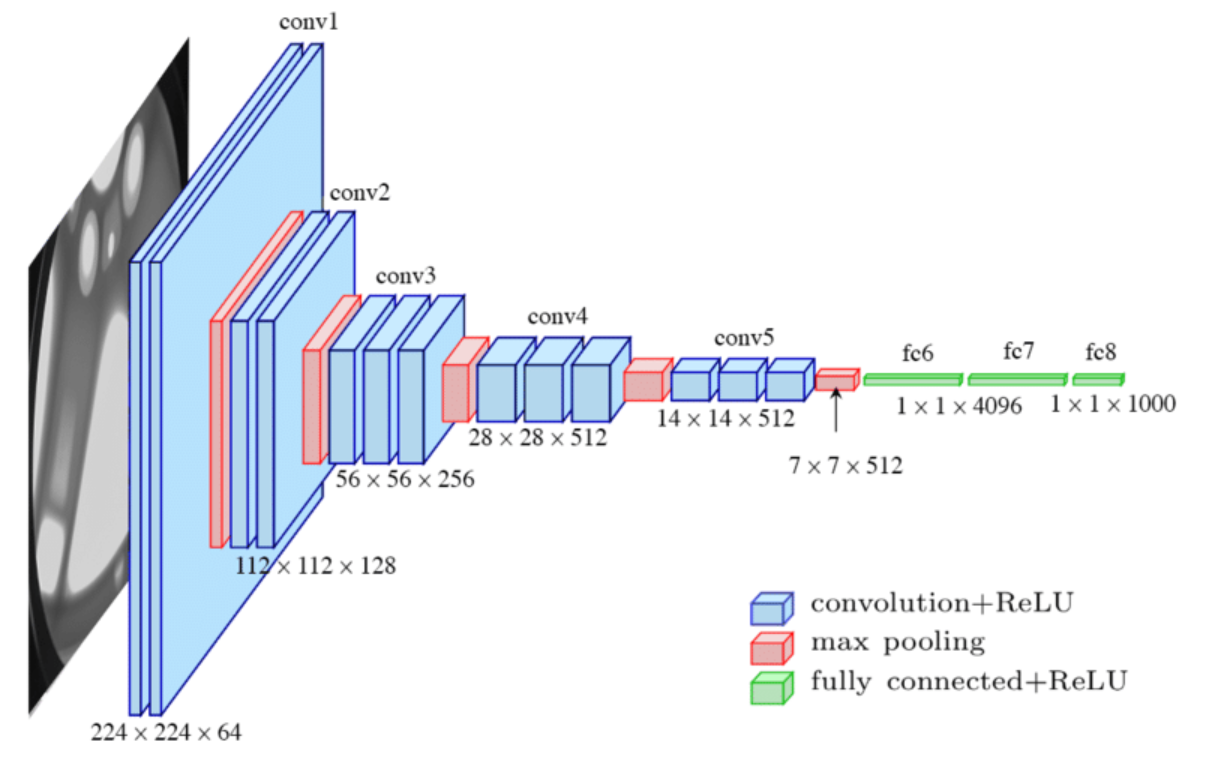
\includegraphics[width=0.8\textwidth,height=0.8\textheight,keepaspectratio]{images/cnn-arch.png}
    \end{figure}
\end{frame}